\documentclass[conference]{IEEEtran}
\usepackage{cite}
\usepackage{amsmath,amssymb,amsfonts}
\usepackage{algorithmic}
\usepackage{graphicx}
\usepackage{textcomp}
\usepackage{xcolor}
\def\BibTeX{{\rm B\kern-.05em{\sc i\kern-.025em b}\kern-.08em
    T\kern-.1667em\lower.7ex\hbox{E}\kern-.125emX}}
\begin{document}

\title{Project: COVID-19 Assisted Diagnosis\\


\author{\IEEEauthorblockN{Frie Van Bauwel\textsuperscript{1}}
\and
\IEEEauthorblockN{Lotte Van de Vreken\textsuperscript{2}}
\and
\IEEEauthorblockN{Marcin Jedrych\textsuperscript{3}}
\and
\IEEEauthorblockN{Xueting Li\textsuperscript{4}}

\and


%\textsuperscript{1} Bachelor of Science in de ingenieurswetenschappen - werktuigkunde-elektrotechniek \hfill\\
%\textsuperscript{2} Bachelor of Science in de ingenieurswetenschappen - biomedische ingenieurstechnieken\hfill\\
%\textsuperscript{3}  Bachelor of Science in de ingenieurswetenschappen - elektrotechniek\hfill}
\textsuperscript{1,2,3,4}  Master of Science in statistical data analysis - computational statistics\hfill}}

\maketitle



\section{Introduction}
Within this project on medical image classification, two deep learning models are trained to classify X-ray images of lungs as COVID-positive or COVID-negative images. Further, the Grad-CAM visualization technique is used to be able to show on which areas of an X-ray image are mainly used by the algorithm to decide whether an image shows a person affected with COVID or a person not affected with COVID. This report describes first how the data are explored, preprocessed and augmented (\ref{sec:task_1}). It then explains how a baseline model, using a convolutional network, was fitted (\ref{sec:task_2}) and how transfer learning was used to make use of the pretrained ResNetV2 model (\ref{sec:task_3}). \ref{sec:task_4} describes in which the Grad-CAM visualisation is used to understand why missclassifications happen in the best performing model trained in the previous tasks.
After the \ref{sec:conclusion}, the report describes how this project was divided between all group members (\ref{sec:author_contributions}. The final section entails our use of generative AI during the project (\ref{sec:generative_AI}).


\section{Task 1: Data Exploration, Pre-Processing and Augmentation}\label{sec:task_1}
Question 1
-	COVID and normal chest X-rays can have subtle visual differences, making it hard for a model to learn the differences between classes.
-	The dataset size is relatively small (only 1600 training images), which increases the risk of overfitting.
-	X-ray images often have variability in terms of brightness, contrast, and anatomical differences between individuals, which introduce noise
-	If the dataset is not perfectly balanced the model might become biased toward the majority class but fortunately, the plot shows that this is not the case here.
Question 2
Based on the pixel statistics and label distribution, the datasets appear to be fairly uniformly divided, though not perfectly. The average pixel values and standard deviations are similar across sets — training (mean ≈ 0.53, std ≈ 0.25), validation (mean ≈ 0.55, std ≈ 0.26), and test (mean ≈ 0.55, std ≈ 0.26) — indicating consistent image intensity. The class distribution also looks well balanced overall. The training set is evenly split, while the validation set shows a slight tilt toward NORMAL, and the test set has a few more COVID samples. These minor differences are not concerning. Overall, the datasets are reasonably well-balanced in terms of both pixel characteristics and label distribution.
Question 3
COVID-19 lesions often appear as ground-glass opacities or consolidation patches, which have different intensity distributions compared to normal lungs.
If these variations between the COVID-positive and normal X-rays are not addressed properly (e.g., by normalization or augmentation), the model could fail to learn the correct patterns, reducing its accuracy. This issue might cause the model to misinterpret lesions as part of normal anatomy or vice versa.Unaccounted-for artifacts can mislead the model by focusing on irrelevant patterns. It’s crucial to ensure that image pre-processing (such as normalization and augmentation) reduces the impact of these artifacts. This would help the model focus on medically relevant features rather than on noise or imaging imperfections.

Question 4
We downsample to from 299x299 to 128x128, this forms a good compromise between not downscalig too much and having doable runtimes of the algorithms.
Downsampling does not only mean you lose some information, it also makes the picture more general, and cause less overfitting of your model.

Question 5
In order to a general method, the images were normalized using dataset statistics. The mean and standarddeviation of all pixels in the training ?XX and validation?? dataset were used as normalization statistics. 
The same statistics could be used over all three channels as all these channels have the same values since the pictures are black and white. It is however not possible to use a loaded image with just one channel in the resnet50v2 model. Hence, the images are loaded as if they have 3 channels.
FYI: featurewise => all images same statistics, samplewise: different statistics each image
Question 6
Excessive transformations could indeed introduce unrealistic patterns. It is for example very unlikely that the images would be vertically flipped, as lungs are not symmetrical: for the vast majority of people, the heart is on the left side of the body causing a smaller lung on that side. 
We also assumed that the pictures were never horizontally flipped, as out of all samples we looked at, there was not one that was flipped there. However, slight rotations, zooms and translations are very relevant as it is likely those occur in the dataset, using these transformations thus generalizes the training data set in a relevant way, which can avoid overfitting of the model in a later stage.

\section{Task 2}
Question 7
I would use Recall and Precision metrics, because misclassifying COVID cases as "normal" (false negatives) could have serious implications,these two metrics would be critical.
Question 8
From the Accuracy picture, we can see that model is overfitting,meaning the model is performing well on the training data but poorly on unseen data. Learning rate would need to be optimized first: To balance training speed and model accuracy.
Question 9


\section{Task 3}

Within task 3, a neural network is built using the transfer learning approach. In other words, a pretrained model is used as a basis to built a model, hereby making it possible to use a network with many layers even though a limited set of training data is available. 
In this case, the ResNet50V2, a model consisting of 50 layers, is used as the pretrained model. After the ResNet50V2 model, four extra layers are added. First, a GlobalAveragePooling2D layer is added to reduce the spatial dimensions. Then, a 128-node dense layer with relu-activation is added in combination with a dropout layer to reduce risk of overfitting. A final single-node dense layer with sigmoid activation was used to get the binary output.

After setting the model architecture, the hyperparameters of the added layers are tuned. The batch size, learning, and dropout rates are tuned. Table XXXXX shows the XXranges/combinations that are used during the hypertuning process and indicated the optimal outcomes for each hyperparameter. 
While tuning the hyperparameters, the pretrained parameters in the ResNet50V2-layers remain unchanged. Early stopping based on the validation loss is used with a patience of five steps. After this tuning step, a model is trained during 16 epochs based on the training and validation data. Another, final, model is trained in which the ResNet50V2-layers are unfrozen, hence fine-tuning the weights in these layers is possible. The training curves of the model before unfreezing the ResNet50V2-layers is visualized in figureXXX, the training curves of the model after unfreezing is visualized in figureXXX


-comparison training curve between 3 models

- results on the test set (confusion matrix)
- discuss why probably better than baseline model (advantages)
-but xxx (disadvantages)
- possibilities to improve plan of attack

Question 13
The dataset was limited so the architecture was chosen so that overfitting will be limited. We chose a GlobalAveragePooling2D layer to reduce spatial dimensions.
To prevent overfitting, a dense layer and dropout layer was added. Finally, a single-node dense layer with sigmoid activation was used to get the binary output.

Question 14

Question 15

Question 16

Question 17
Transfer learning requires less training data and converges faster. 
The pretrained model is not trained specifically on X-ray data.

Question 18
We could use a model that was specifically trained on medical images such as CheXNet.
We could combine this approach with semi-supervised learning with unlabeld X-rays.

\section{Task 4}

Question 19

Did you have to modify the algorithm to account for a scalar output? If so, how did you modify it?

Yes, we modified the model to use a dense layer with two outputs, providing a score for each class (COVID and normal), to align with Grad-CAM’s requirement for class-specific outputs.

Question 20

Do you think that having only two class labels affects the explanation? If you do, how so?

Initially, the model produced a single scalar output indicating whether the image was classified as COVID or not.
After the modification, the model outputs logits (or probability scores) for both classes separately. The class with the highest score is chosen, which is still equivalent to binary classification, but the explanation now considers both classes individually.

Question 21

Do the Grad-CAM visualizations highlight medically relevant areas in the X-ray, such as lung opacities or other features indicative of COVID-19?

Yes, when setting pred\_index to zero (corresponding to the COVID class), the Grad-CAM visualizations show that the model focuses on lung areas, which are medically relevant and consistent with clinical expectations.
Question 22

The Grad-CAM visualizations revealed some activation outside the lungs, sometimes focusing on a square region unrelated to the disease. This suggests that the model may have learned to rely on spurious features, indicating potential biases.
We can observe activation sometimes to a square area in the image, which is not relevant for the classification.

Question 23

Was Grad-CAM useful for understanding the model’s misclassifications?

no answer yet

Question 24

Consider a scenario in which you can collect additional data and retrain the model. Would you change anything based on the Grad-CAM explanations?

no answer yet

\subsection{Subsection 1 (e.g. Methods)}
 Details the strategies you have employed, including those that did not work.

\subsection{Subsection 2 (e.g. Results)}
Includes tables with quantitative results (Table~\ref{table:example}) and images (Fig.~\ref{fig:example}) from your project while carefully explaining their meaning and how you produced them.
\begin{table}[htbp]
\caption{Table Type Styles}
\begin{center}
\begin{tabular}{|c|c|c|c|}
\hline
\textbf{Table}&\multicolumn{3}{|c|}{\textbf{Table Column Head}} \\
\cline{2-4} 
\textbf{Head} & \textbf{\textit{Table column subhead}}& \textbf{\textit{Subhead}}& \textbf{\textit{Subhead}} \\
\hline
copy& More table copy$^{\mathrm{a}}$& &  \\
\hline
\multicolumn{4}{l}{$^{\mathrm{a}}$Sample of a Table footnote.}
\end{tabular}
\label{table:example}
\end{center}
\end{table}

\begin{figure}[htbp]
\centerline{
\includegraphics{fig1.png}}
\caption{Example of a figure caption.}
\label{fig:example}
\end{figure}
\subsection{Subsection 3 (e.g. Discussion)}
Discusses the results and your general experience with the project, as well as provide answers to the questions about the task.
\section{Task 2: Building the baseline model}
\section{Task 3: Transfer Learning}
\section{Task 4: Explainability through Grad-CAM}

To better understand the decisions made by our COVID-19 classifier, we did a Gradient-weighted Class Activation Mapping (Grad-CAM). Grad-CAM is a technique that highlights the regions of an input image that contribute most strongly to a model’s decision. It works by computing the gradient of a target class score with respect to the activations of the final convolutional layer. These gradients are averaged spatially to obtain importance weights, which are then combined with the activation maps to generate a heatmap that can be overlaid on the original image.
Initially, the model's scalar output directly indicated a binary decision. However, Grad-CAM requires class-specific outputs. Therefore, we replaced the final layer with a dense layer producing two logits—one for each class (COVID and normal). After this adjustment, the model generated separate scores for both classes, with the predicted class corresponding to the higher score. As a result, the fundamental decision-making process of the model remained unchanged.
Applying Grad-CAM to test samples showed that, when focusing on the COVID-19 class, the visualizations predominantly highlighted the lung regions—consistent with clinical expectations, given that lung opacities are a key indicator of COVID-19 on chest X-rays. However, Grad-CAM also revealed potential model biases: in some cases, activations appeared outside the lungs, often around rectangular artifacts. These findings highlight that the model may have learned spurious, non-disease-related features, which underlines the purpose of Grad-CAM in explaining and evaluating the model's behavior.
Our Grad-CAM implementation follows the Keras official tutorial \cite{keras_gradcam}, adapting it to our model. Using TensorFlow’s \texttt{GradientTape}, we computed the gradient of the selected class score with respect to the convolutional feature maps. The gradients were averaged over the spatial dimensions to weigh the importance of each feature channel, and the resulting weighted activation maps were aggregated to form the Grad-CAM heatmap. Finally, the heatmap was normalized between 0 and 1 for visualization.
\begin{figure}[h] \centering 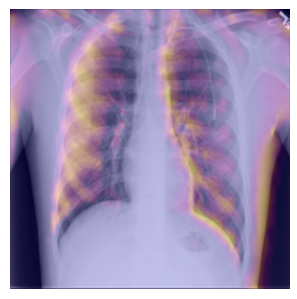
\includegraphics[width=0.8\columnwidth]{gradcam_example.png} \caption{Example Grad-CAM heatmap highlighting lung regions associated with a COVID-positive classification.} \label{fig:gradcam_example} \end{figure}

\+Question 23 \& 24

\section{Conclusions}
\section{Author contributions and collaboration}
\section{Use of Generative AI}


\subsection{Figures and Tables}
\paragraph{Positioning Figures and Tables}




\section*{References}
Example References:
\begin{thebibliography}{00}
\bibitem{b1} G. Eason, B. Noble, and I. N. Sneddon, ``On certain integrals of Lipschitz-Hankel type involving products of Bessel functions,'' Phil. Trans. Roy. Soc. London, vol. A247, pp. 529--551, April 1955.
\bibitem{b2} J. Clerk Maxwell, A Treatise on Electricity and Magnetism, 3rd ed., vol. 2. Oxford: Clarendon, 1892, pp.68--73.
\bibitem{b3} I. S. Jacobs and C. P. Bean, ``Fine particles, thin films and exchange anisotropy,'' in Magnetism, vol. III, G. T. Rado and H. Suhl, Eds. New York: Academic, 1963, pp. 271--350.
\bibitem{b4} K. Elissa, ``Title of paper if known,'' unpublished.
\bibitem{b5} R. Nicole, ``Title of paper with only first word capitalized,'' J. Name Stand. Abbrev., in press.
\bibitem{b6} Y. Yorozu, M. Hirano, K. Oka, and Y. Tagawa, ``Electron spectroscopy studies on magneto-optical media and plastic substrate interface,'' IEEE Transl. J. Magn. Japan, vol. 2, pp. 740--741, August 1987 [Digests 9th Annual Conf. Magnetics Japan, p. 301, 1982].
\bibitem{b7} M. Young, The Technical Writer's Handbook. Mill Valley, CA: University Science, 1989.
\end{thebibliography}
\end{document}
